\section{Isochrone Fitting}\label{sec:isoFit}
We fit pairs of isochrones to the HUGS data for NGC 2808 using \fidanka, as
descrbed in \S \ref{sec:fidanka}. Two isochrones, one for Population A and one
for Population E are fit simultaneously. These isochrones are constrained to
have distance modulus, $\mu$, and color excess, E(B-V) which agree to within
0.5\% and an ages which agree to within 1\%. Moreover, we constrain the mixing length, $\alpha_{ML}$, for any two
isochrones in a set to be within 0.5 of one and other. For every isochrone in
the set of combination of which fulfilling these constraints $\mu$, $E(B-V)$,
Age$_{A}$, and $Age_{B}$ are optimized to reduce the $\chi^{2}$ distance
($\chi^{2} = \sum\sqrt{\Delta \text{color}^{2} + \Delta \text{mag} ^{2}}$)
between the fiducial lines and the isochrones. Because we fit fiducial lines
directly, we do not need to consider the binary population fraction, $f_{bin}$,
as a free parameter.

The best fit isochrones are shown in Figure \ref{fig:BestFitResults} and
optimized parameters for these are presented in Table \ref{tab:BestFitResults}.
We find helium mass fractions that are consistent with those identified in past
literature \citep[e.g.][]{Milone2015}. Note that our helium mass fraction grid
has a spacing of 0.03 between grid points and we are therefore unable to
resolve between certain proposed helium mass fractions for the younger sequence
(for example between 0.37 and 0.39).

\begin{figure*}
  \centering
  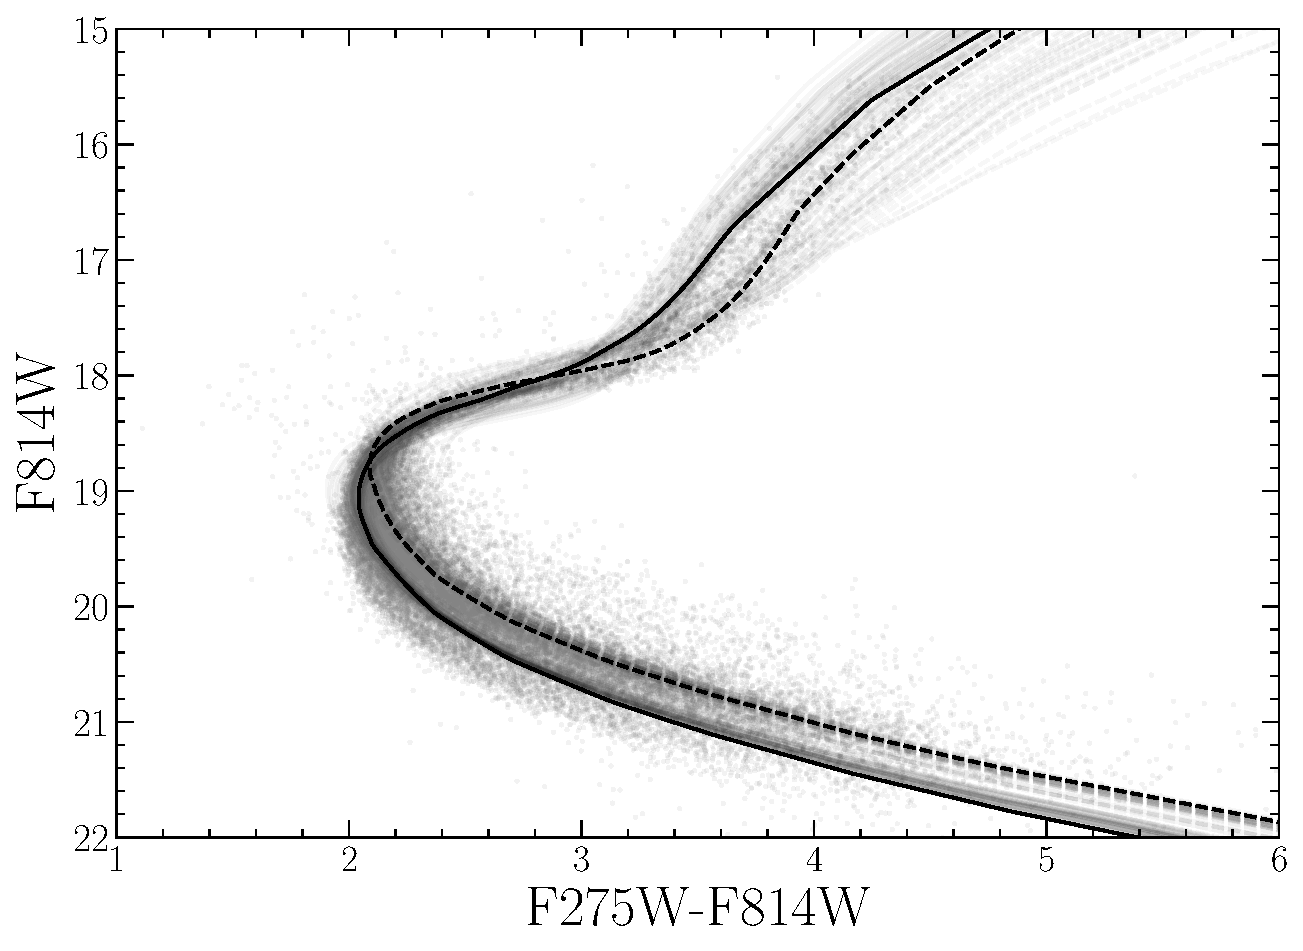
\includegraphics[width=0.9\textwidth]{BestFitResults.pdf}
  \caption{Best fit isochrone results for NGC 2808. The best fit population A
  and E models are shown as black lines. The following 50 best fit models are
  presented as grey lines. The solid black line is fit to population A, while
  the dashed black line is fit to population E.}
  \label{fig:BestFitResults}
\end{figure*}

\begin{table*}
  \centering
  \begin{tabular}{c | c c c c c c}
    \hline
    Population & Age & Distance Modulus & Extinction & Y & $\alpha_{ML}$ & $\chi^{2}_{\nu}$\\
    & [Gyr] & & [mag] & & &\\
    \hline
    \hline
    A & 12.996$^{+0.87}_{-0.64}$ & 15.021 & 0.54 & 0.24 & 2.050 & 0.021\\
    E & 13.061$^{+0.86}_{-0.69}$ & 15.007 & 0.537 & 0.39 & 1.600 & 0.033 \\
    \hline
  \end{tabular}
  \caption{Best fit parameters derived from fitting isochrones to the fiducual lines derived from the NCG 2808 photometry. The one sigma uncertainty reported on population age were determined from the 16th and 84th percentiles of the distribution of best fit isochrones ages.}
  \label{tab:BestFitResults}
\end{table*}


Past literature \citep[e.g. ][]{Milone2015, Milone2018} have found helium mass
fraction variation from the low redmost to bluemost populations of $\sim 0.12$.
Here we find a helium mass fraction variation of 0.15 which, given the spacing
of the helium grid we use \textbf{is consistent with these past results}.

\subsection{The Number of Populartions in NGC 2808}
In order to estimate the number of populations which ideally fit the NGC 2808
F275W-F814W photometry without overfitting the data we make use of silhouette
analysis \citep[][and in a similar manner to how \citet{Valle2022} preform
their analysis of spectroscopic data]{ROUSSEEUW198753}. We find the average
silhouette score for all tagged clusters identified using BGMM in all magnitude
bins over the CMD using the standar python module \texttt{sklearn}. Figure
\ref{fig:clusterAn} shows the silhouette analysis results and that two
populations fit the photometry most ideally. This is in line with what our BGMM
model predicts for the majority of the the CMD.

\begin{figure}
  \centering
  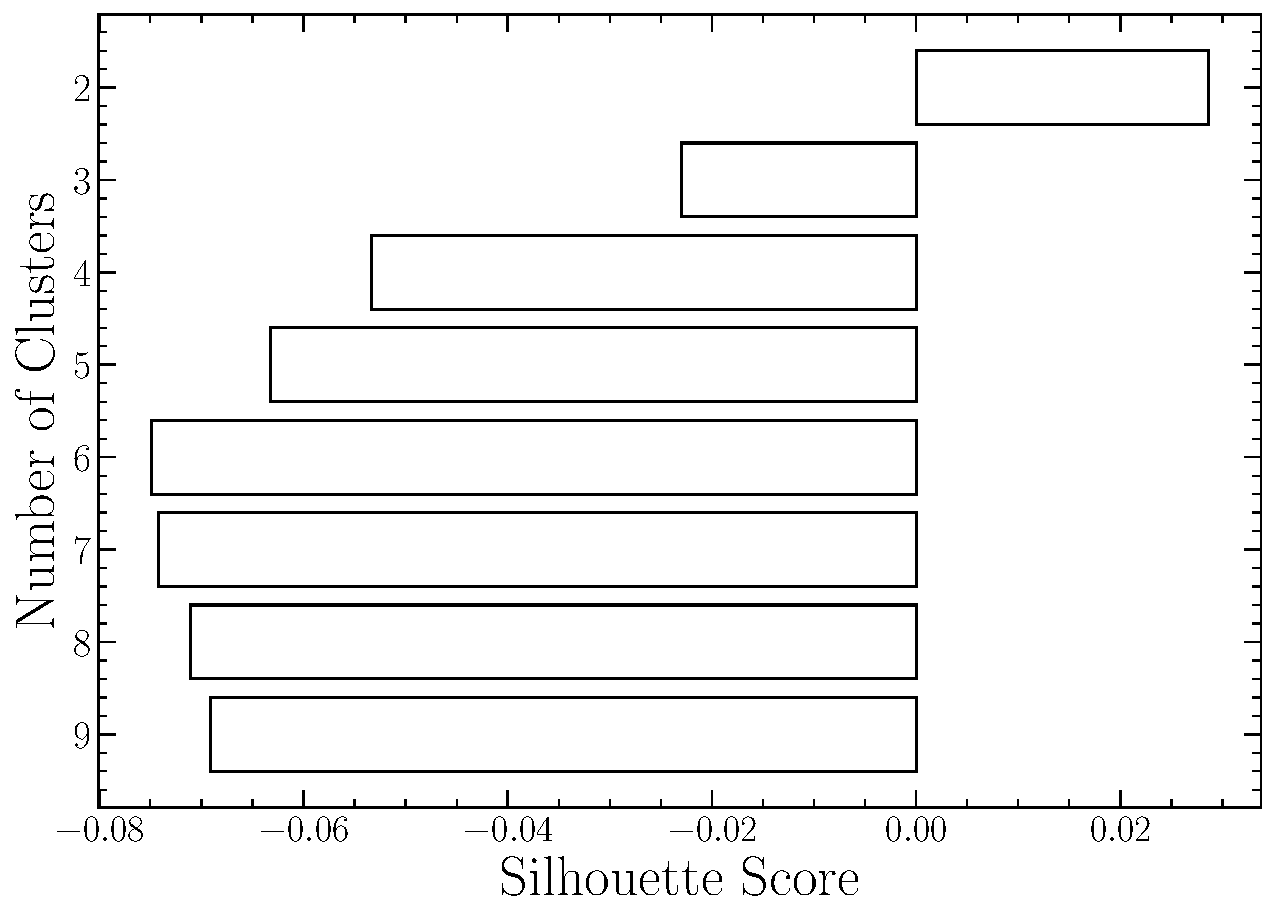
\includegraphics[width=0.45\textwidth]{ClusterAnalysis.pdf}
  \caption{Silhouette analysis for NGC 2808 F275W-F814W photometry. The Silhouette scores
  are an average of score for each magnitude bin. Positive scores incidate that the clustering
  algorithm produced well distinguised clusters while negative scores indicate clusters which are not
  well distinguised.}
  \label{fig:clusterAn}
\end{figure}


\subsection{ACS-HUGS Photometric Zero Point Offset}
The Hubble legacy archive photometry used in this work is calibrated to the
Vega magnitude system. However, we have found that the photometry has a
systematic offset of $\sim0.026$ magnitudes in the F814W band when
compared to the same stars in the ACS survey (Figure \ref{fig:offset}). The
exact cause of this offset is unknown, but it is likely due to a difference in
the photometric zero point between the two surveys. A full correction of this
offset would require a careful re-reduction of the HUGS photometry, which is
beyond the scope of this work. We instead recognize a 0.02 inherent uncertainty
in the inferred magnitude of any fit when comparing to the ACS survey. This
uncertainty is small when compared to the uncertainty in the
distance modulus and should not affect the conclusion of this
paper. 

\begin{figure*}
  \centering
  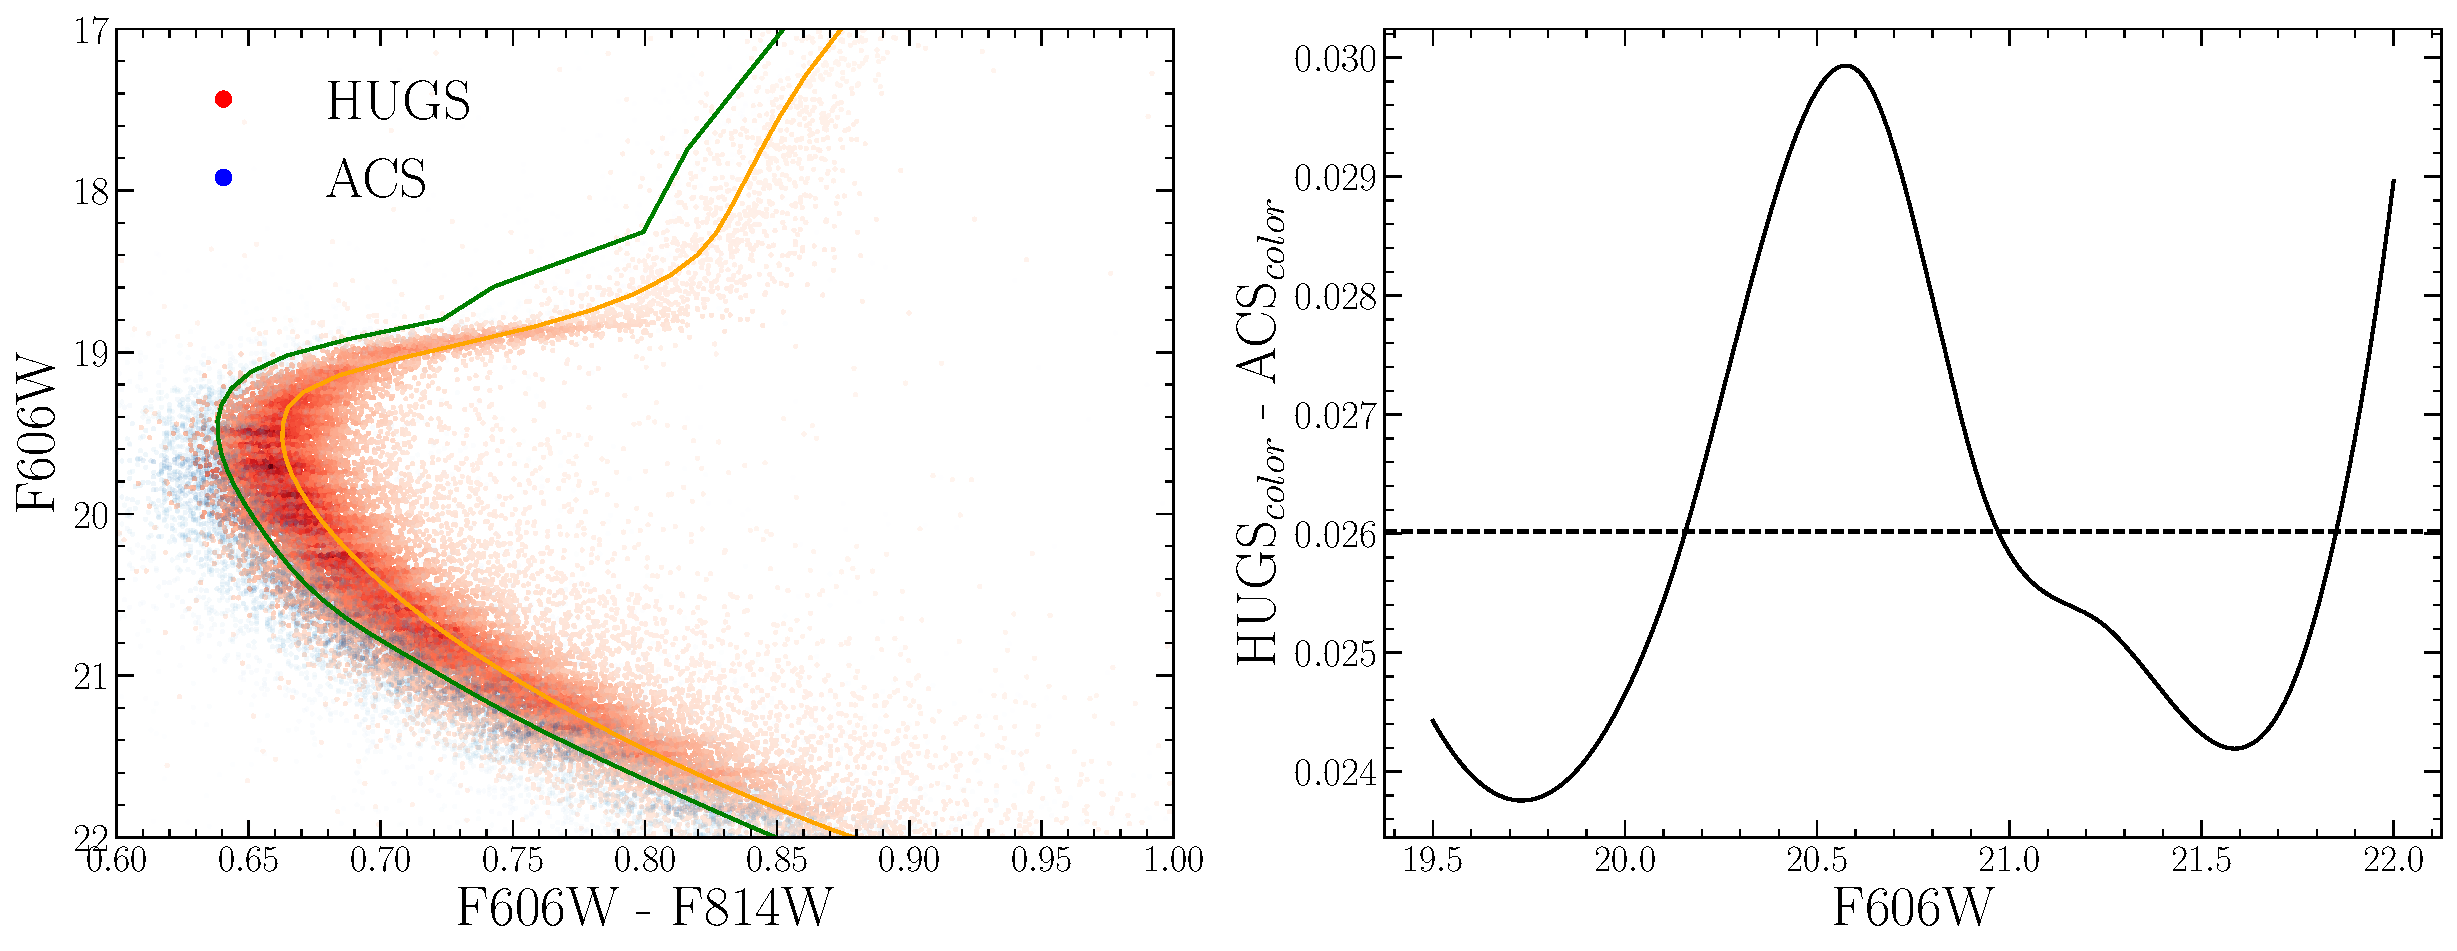
\includegraphics[width=0.90\textwidth]{photometricOffset.pdf}
  \caption{(left) CMD showing the photometric offset between the ACS and HUGS data for NGC 2808. CMDs have been randomly subsampled and colored by point density for clarity. (right) Mean difference between the color of the HUGS and ACS fiducual lines at the same magnitude. Note that the ACS data is systematically bluer than the HUGS data.}
  \label{fig:offset}
\end{figure*}

The oberved photometric offset between ACS and HUGS reductions introduces a
systematic uncertainity when comparing parameters derived from isochrone fits
to ACS data vs those fit to HUGS data. Specifically, this offset introduces a
$\sim 2 Gyr$ uncertainity when comparing ages between ACS and HUGS. Moreover,
for two isochrone of the same age, only seperated by helium mass fraction, a
shift of the main sequence turn off of is also expected. Figure \ref{fig:HeMO}
shows this shift. Note a change in the helium mass fraction of a model by 0.03
results in an approximate 0.08 magnitude shift to the main sequence turn off
location. This means that the mean 0.026 magnitude offset we find in between
ACS and HUGS data corresponds to an additional approaximate 0.01 uncertainity
in the derived helium mass fraction when comparing between these two datasets. 

\begin{figure}
  \centering
  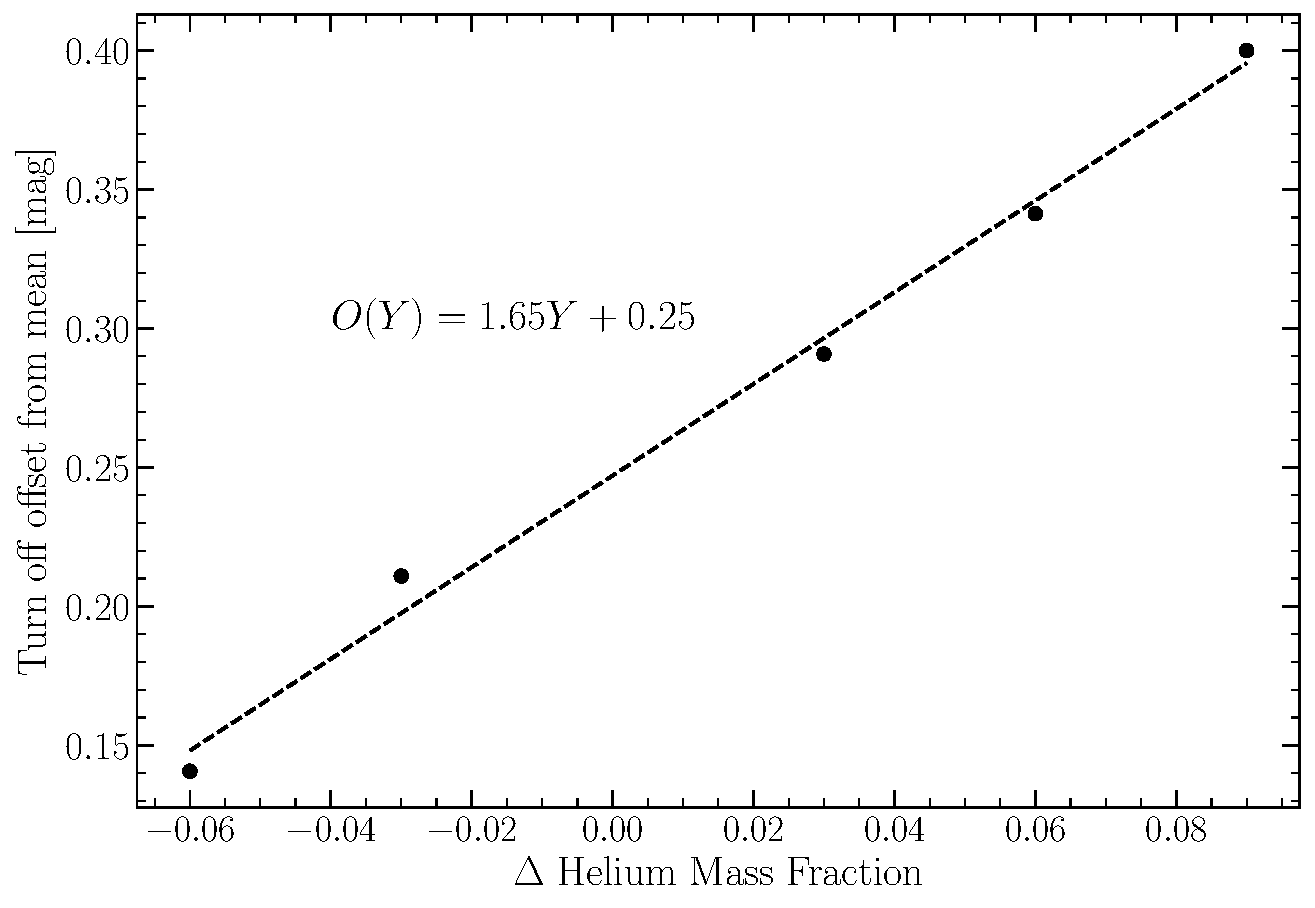
\includegraphics[width=0.45\textwidth]{HeliumMeanOffset.pdf}
  \caption{Main sequence turn off magnitude offset from a guage helium mass fraction (Y=0.30 chosen). All main sequence turn off locations are measured at 12.3 Gyr {\color{blue} Should I make these contour surfaces for various ages?}}
  \label{fig:HeMO}
\end{figure}
